\documentclass{article}

\usepackage{polski}
\usepackage[utf8]{inputenc}
\usepackage{graphicx}

\title{Dokumentacja projektowa}
\date{2018-03-18}
\author{Jędrzej Kozal}

\begin{document}

\begin{titlepage}
	\centering
	
\includegraphics[width=0.25\textwidth]{logo_pol_wroclaw.png}\par\vspace{1cm}
	{\scshape\LARGE Politechnika Wrocławska \par}
	\vspace{1cm}
	{\scshape\Large Zastosowanie informatyki w gospodarce\par}
	\vspace{1.5cm}
	{\huge\bfseries Aplikacja do rezerwacji miejsc w restauracjach \par}
	\vspace{2cm}
	{\Large\itshape Hubert Duś\par}
	{\Large\itshape Jędrzej Kozal\par}
	{\Large\itshape Eliza Mocek\par}
	{\Large\itshape Piotr Montewka\par}

	\vfill
	prowadzący\par
	Dr inż.~Marek \textsc{Woda}

	\vfill

% Bottom of the page
	{\large 2018-03-18\par}
\end{titlepage}


\section{Wstęp}

\subsection{Cel projektu}
Celem projektu realizowanego w ramach kursu, jest stworzenie aplikacji biznesowej, umożliwiającej rezerwacje miejsc w wybranych restauracjach. Zakłada się, że tworzona aplikacja będzie umożliwiała rezerwację miejsc w restauracji w porozumieniu z właścicielem i obsługą. Analogicznym pomysłem może być rezerwacja miejsc w kinie, która najczęściej odbywa się drogą elektroniczną. Tworzona aplikacja ma ułatwić pracę restauratorom i pozwolić na lepsze zarządzanie dostępnym miejscem oraz pośrednio zaopatrzeniem i personelem.

Ponadto istotnym celem projektu, jest zapoznanie się z realiami pracy nad dużym projektem informatycznym oraz analiza i próba rozwiązania podstawowych problemów jakie są związane z tym zagadnieniem. Projekt może być wymagający na poziomie technicznym, jak i komunikacyjnym. Przed przystąpieniem do aktywności zawodowej nie jest łatwo zdobyć doświadczenie w zakresie pracy w większym zespole inżynierskim.
\subsection{Zakres projektu}
Podstawowy zakres funkcjonalności można rozważać z perspektywy klienta, chcącego zamówić miejsce w restauracji, oraz właściciela i obsługi rezerwacji. Klient dzięki aplikacji powinien mieć zdolność zarezerwowania miejsca w wybranej przez siebie restauracji. Restauratorzy powinni mieć zdolność dodawania własnych rezerwacji oraz potwierdzania rezerwacji danych użytkowników. Aplikacja ma ułatwić i zautomatyzować komunikację między klientami a restauracjami. Warto zaznaczyć, że aplikacja nie udostępnia narzędzi umożliwiających zarządzanie restauracjami. W celu osiągnięcia przedstawionego celu należy stworzyć stronę internetową umożliwiającą dostęp do wybranych funkcjonalności, połączoną z aplikacją webową z dostępem do bazy danych.



\section{Analiza wymagań}

\subsection{Analiza rynkowa}
Potencjalna grupa docelowa odbiorców?
\subsubsection{Dostępne rozwiązania}

Na rynku jest dostępnych kilka aplikacji oferujących zbliżony zakres funkcjonalności do przedstawionego. Poniżej przedstawiono pobieżną analizę dostępnych rozwiązań.

\paragraph{gastrobooking.pl}
Popularny w polsce serwis do rezerwacji miejsc w restauracjach. W Polsce umożliwia rezerwację stolików jedynie w Krakowie. 

\paragraph{quandoo.com}


\paragraph{zomato.com}

\paragraph{opentable.com}
Jest to aplikacja posiadająca najwięszką bazę restauracji (40 000) w 14 krajach. Na Polskim rynku dostępne są jedynie dwie restauracje. 

\subsubsection{Analiza wymagań biznesowych}

Wymienione w poprzednim paragrafie serwisy nie występują w Polsce, lub są słabo rozpowszechnione. W porównaniu do konkurencji podstawową zaletą aplikacji ma być jej niska cena, oraz prostota. Zwiększa to zakres firm, który mogłyby sobie pozwolić na wdrożenie naszej aplikacji, co na dłuższą metę może stanowić o większej popularności.

Główną grupą docelową naszego produktu są restauratorzy oraz obsługa restauracji z dużą liczbą rezerwacji. Dzięki przygotowanej aplikacji mogą skorzystać z najnowszych rozwiązań technicznych, aby lepiej zarządzać swoją dostępnymi miejscami, oraz personelem. Zintegrowanie opracowanego systemu z innymi systemami umożliwiającymi zarządzanie personelem, kosztami czy zamówieniami znacząco ułatwiałoby zarządzanie i podejmowanie właściwych decyzji na poziomie managerskim. 


\subsection{Wymagania funkcjonalne}

\begin{figure}
\centering
	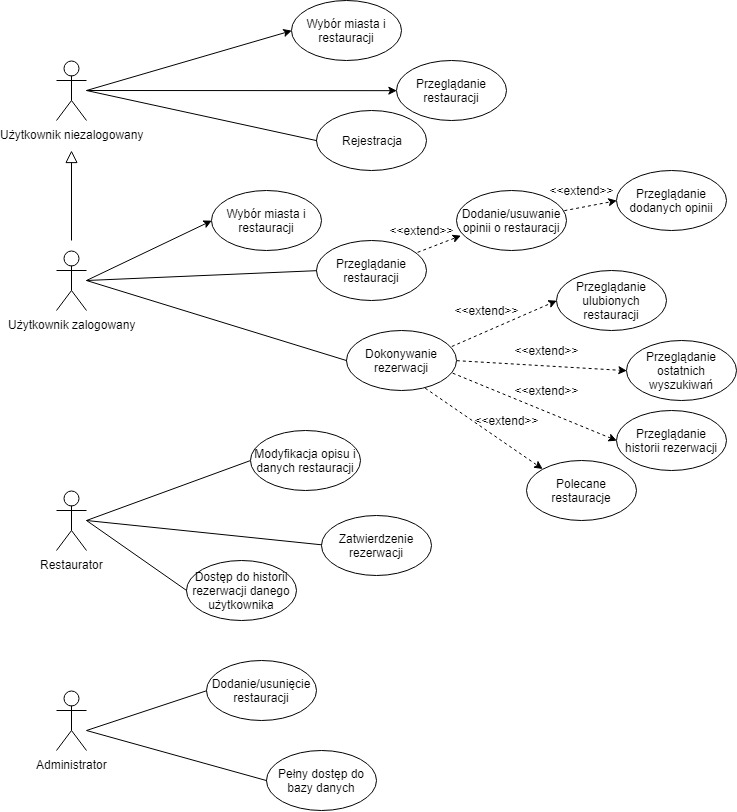
\includegraphics[width=0.90\textwidth]{use_case.jpg}
	\caption{Schemat przypadków użycia systemu.}
\end{figure}

\subsubsection{Podstawowe przypadki użycia}



\subsection{Wymagania niefunkcjonalne}

\subsubsection{Wykorzystane technologie i narzędzia}

Projekt został zrealizowany z wykorzystaniem języka C\# oraz frameworka ASP.NET MVC. Do realizacji frontendu zostały wykorzystane HTML5, CSS 3.0 oraz JavaScript. Jako system zarządzania bazą danych wykorzystano Microsoft SQL Server.

\begin{figure}
\centering
		\begin{minipage}{2cm}
			
\includegraphics[width=2cm]{c_hasztag.png}
		\end{minipage}
		\begin{minipage}{2cm}
			
\includegraphics[width=2cm]{asp_net-MVC.png}
		\end{minipage}
		\begin{minipage}{2cm}
			
\includegraphics[width=2cm]{html.png}
		\end{minipage}
		\begin{minipage}{2cm}
			
\includegraphics[width=2cm]{sql.png}
		\end{minipage}
	\caption{Wykorzystane technologie.}
	\label{fig:technologie}
\end{figure}

\begin{figure}
\centering
	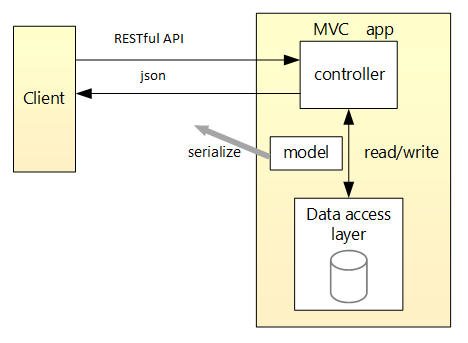
\includegraphics{mvc.png}
	\caption{Podstawowy schemat działania aplikacji korzystającej z .NET MVC.}
\end{figure}

\subsubsection{Wykorzystane dobre praktyki}

W trakcie projektu przyjęto metodologię SOLID, oraz fragmenty metodologii Clean Code. Pozwala to na stworzenie łatwo rozszerzalnego kodu, który jest utrzymywalny i dobrze zorganizowany.

\section{Projekt systemu}

\subsection{Architektura systemu}

W niniejszym rozdziale przedstawiono ogólny przegląd architektury całej aplikacji, opartej na zalecanych sposobach pracy z wybranymi narzędziami.

\subsubsection{ASP.NET MVC}

Projekty wykonywane w frameworku ASP.NET MVC wymuszają pewną organizację projektu, która zwiększa uporządkowanie oraz wymusza korzystanie z dobrych praktyk. W projekcie można wyróżnić 4 zasadnicze części: Views, Controllers, Models i Router. Poniżej przedstawiono krótki opis poszczególnych części.

\paragraph{Model}
Modele są odpowiedzialne za przechowywanie informacji domenowej i stanu aplikacji. Najczęściej są implementowane jako Plain Old CLR Object (POCO) i służą do modelowania danych z bazy. Obiekty te są niezależne od frameworków, systemu zarządzania bazą danych czy mapowań ORM. Modele mogą być łączone w ViewModele, aby ułatwić grupowanie i przekazywanie informacji w aplikacji.

\paragraph{View}
Jest to frontendowa część projektu, która determinuje wygląd strony pokazywanej użytkownikowi. Technologie wykorzystywane w tym obszarze to HTML, CSS oraz JavaScript. Dodatkowo do widoku są przesyłane dane z innych komponentów w postaci modeli lub viewmodeli. ASP.NET MVC umożliwia dodawanie fragmentów kodu w C\# do ułatwienia wykorzystywania danych z modeli.

\paragraph{Controler}
Najczęściej jest to element implementujący wybraną część logiki biznesowej. Wykorzystuje dane z Modeli, aby wytworzyć i przekierować użytkownika do odpowiedniego Widoku. Każdy controler jest odpowiedzialny za obsługę HTTP Request. Taka organizacja wymusza podział projektu na mniejsze klasy z dobrze zdefiniowanym zakresem odpowiedzialności.

\paragraph{Router}
Jest to komponent, który odpowiada za mapowanie zapytań HTTP na poszczególne akcje w kontrolerach.
\\\\
Pierwsze trzy komponenty są dobrze znane ze wzorca projektowego na Model-View-Controler, natomiast ostatni jest często spotykanym dodatkiem w wielu frameworkach sieciowych, umożliwiający łatwe mapowanie. Konstrukcja frameworku MVC pozwala na łatwe rozdzielenie odpowiedzialności komponentów i klas oraz wstrzykiwanie zależności do poszczególnych klas.

\subsubsection{Onion architecture}

\begin{figure}
\centering
	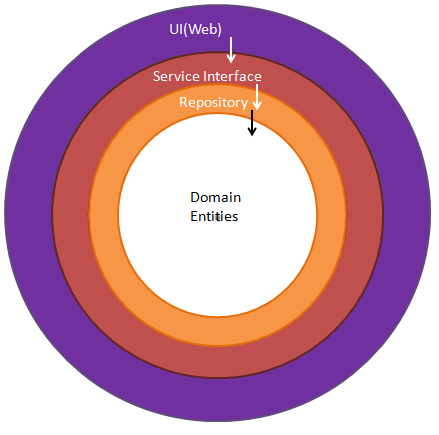
\includegraphics[width=0.50\textwidth]{onion.png}
	\caption[caption]{Warstwy w onion architecture.\\\hspace{\textwidth}Źródło: https://www.c-sharpcorner.com/article/onion-architecture-in-asp-net-core-mvc/}
	\label{fig:onion}
\end{figure}

Onion architecture jest typem architektury mający ułatwić uniknięcie silnych powiązań w kodzie (angl. tightly coupling). Projekt aplikacji wykorzystujący wzorzec Model-View-Controller pozwala łatwo rozdzielić odpowiedzialności między klasy i komponenty, ale nie rozwiązuje problemu mocnych powiązań.

W założeniu aplikacja dzieli się na kilka warstw, które zostały przedstawione na rysunku \ref{fig:onion}. Cała koncepcja opiera się mocno na Dependency inversion (D z mnemonika SOLID). Najbardziej wewnętrzną warstwę tworzą Domain Entities, które przechowują informację na temat obiektów związanych z domeną aplikacji. Implementowane w postaci obiektów POCO  pozwalające na wydobywanie informacji z frameworków ORM. Obiekty te nie powinny być zależne od innych, jednocześnie mogą być wykorzystywane w komunikacji między innymi komponentami, stąd stanowią centrum onion architecture. Repository Layer odpowiada za stworzenie abstrakcji oddzielającej logikę biznesową od danych z poprzediej wartswy. Najbardziej zewnętrzne warstwy oprogramowania to Service Layer zawierająca logikę biznesową oraz UI Layer odpowiadająca za komunikację z użytkownikiem.


\subsection{Projekt frontendu}
Do zdecydowania, czy ta sekcja powinna być zawarta w dokumentacji.
Co mogłoby się w niej znaleźć:
Ogólne overwiev, jakie ma być user expierience, jakaś idea stojąca za projektem frontendu?

\subsection{Projekt bazy danych}
To do:
Schemat tabel

\section{Podsumowanie i wnioski}


\newpage
\begin{thebibliography}{9}

\bibitem{oficjalna strona}
Oficjalna strona ASP.NET MVC
\\\texttt{https://www.asp.net/mvc}

\bibitem{oficjalna dokumentacja}
Oficjalna dokumentacja ASP.NET MVC
\\\texttt{https://docs.microsoft.com/pl\-pl/aspnet/\#pivot\=core\&panel\=core\_overview}

\bibitem{organizacja projektu}
Mosh Hamedani
\textit{Should you split your ASP.NET MVC project into multiple projects?}.
\\\texttt{https://programmingwithmosh.com/csharp/should-you-split-your\\-asp-net-mvc-project-into-multiple-projects/}

\bibitem{organizacja projektu}
Sandeep Singh Shekhawat
\textit{Onion Architecture In ASP.NET Core MVC}
\\\texttt{https://www.c-sharpcorner.com/article/onion-architecture-in-\\asp-net-core-mvc/}

\end{thebibliography}



\end{document}